\documentclass[a4paper,12pt]{article}
\usepackage{czech}
\usepackage[utf8]{inputenc}
\usepackage{a4wide}
\usepackage[dvipdfm]{graphicx}
\usepackage{graphics}
\usepackage{indentfirst}
\usepackage{fancyhdr}
\usepackage{setspace}
\usepackage{amsmath}
\usepackage{amssymb}
\usepackage{epsfig}

%%\usepackage{nopageno}
%%\usepackage{txfonts}
\usepackage[usenames]{color}

\begin{document}

\section{Úkol}
\begin{enumerate}
\item Ze změřeného ohybového obrazce zobrazeného na milimetrovém papíru určete mřížkovou konstantu mřížky.
\item Pomocí aparatury proměřte ohybové obrazce: mřížky, 2 vybraných štěrbin, 2 vybraných dvojštěrbin. Zpracováním měření určete parametry použitých difrakčních prvků.
\item Okalibrujte mikroskopový okulár metodou postupných měření a lineární regresí, odhadněte relativní chybu kalibrace.
\item Mikroskopem změřte parametry všech použitých difrakčních prvků.
\item Výsledky měření v úkolech č.1, č.2 a č.4 srovnejte a diskutujte, v kterém případě jsou spočtené parametry zatíženy nejmenší chybou. 
\end{enumerate}

\section{Teorie}
\subsection{Oprická mřížka}
Optická mřížka je optická součástka sloužící k ohybu světla. Tento ohyb je svázán rovnicí
\begin{eqnarray}
\sin\varphi=\frac{k\lambda}{a},
\end{eqnarray}
kde $\varphi$ je úhel pod kterým vychází kolmo dopadající paprsek, $k$ přiroené číslo a $a$ vzálenost mezi vrypy na mřížce. 
Mřížková konstanta se definuje jako převrácená hodnota $a$.

\subsection{Štěrbina a dvojstěrbina}
Dle \cite{maly} dochází na stětbinách také k ohybu. Vlivem drahových rozdílů následně vzniká na stínítku interferenční obrazec. 
Pro štěrbinu platí
\begin{eqnarray}
I=I_0\frac{\sin^2(\frac{\pi b}{\lambda}\sin\varphi)}{(\frac{\pi b}{\lambda}\sin\varphi)^2},
\label{St}
\end{eqnarray}
kde $I_0$ je maximum, které nastává pro úhel $\varphi = 0$, $b$ je šířka stěrbiny.

Pro dvojštěrbinu výraz podobný
\begin{eqnarray}
I=I_0\frac{\sin^2(\frac{\pi b}{\lambda}\varphi)}{(\frac{\pi b}{\lambda}\varphi)^2}\cos^2\left(\frac{\pi a}{\lambda}\varphi\right),
\label{DSt}
\end{eqnarray}
kde $a$ je vzdálenost středů stěrbin.

\section{Měření}
\subsection{Mřížková konstanta}
Po nastavení stínítka do ohniska čočky v aparatuře (f = 1 m) jsem na milimetrový papír zanesl ohybový obrazec vzniklý ze mnou požité mřížky. 
Odečtené hodnoty jsou vzhledem k bodu nultého řádu v tabulce \ref{TU1} včetně dopočteného průberu a odpovídající mřížkové konstantě ($\lambda = 632.8$ nm).

\begin{table}
$$
\begin{array}{|c|c|c|c|c|}
\hline
k&  x_{k1}/\mbox{mm}&  -x_{k2}/\mbox{mm}&   x_k/\mbox{mm}& a^{-1}/\mbox{mm}^{-1}  \\ \hline
1&  13.0 \pm 0.5 & 12.0 \pm 0.5&    13 \pm 1&   20\pm 2 \\ \hline
2&  25.5  \pm 0.5  & 25.0\pm 0.5&   25\pm 1&    20\pm 2 \\ \hline
3&  38.0 \pm 0.5&    37.0\pm 0.5&   38\pm 1&    20\pm 2 \\ \hline
4&  50.5 \pm 0.5&  49.0\pm 0.5& 50\pm 1&    20\pm 2 \\ \hline
5&  63.0 \pm 0.5&  62.0\pm 0.5& 63\pm 1&    20\pm 2 \\ \hline
6&  75.0 \pm 0.5&  75.0\pm 0.5& 75\pm 1&    20\pm 2 \\ \hline
7&  88.0 \pm 0.5&  87.0\pm 0.5& 88\pm 1&    20\pm 2 \\ \hline
8&  100.0 \pm 0.5& 100.0\pm 0.5&    100\pm 1&   20\pm 2 \\ \hline
9&  103.0 \pm 0.5& 103.0\pm 0.5&    103\pm 1&   18\pm 2 \\ \hline
10& 116.0\pm 0.5&  115.0\pm 0.5&    116\pm 1&   18\pm 2 \\ \hline
\end{array}
$$
\caption{Výsledky měření mřížky s pomocí milimetrového papíru.}
\label{TU1}
\end{table}

Po statistickém vyhodnocení a vypuštěním dvou posledních naměřených hodnot (z důvodu vyšší nepřesnosti při odečítání) jsem získal mřížkovou konstantu
\begin{eqnarray}
a^{-1}=(20\pm 1)\mbox{mm}^{-1}
\end{eqnarray}
Dominantní složka chyby byla nepřesnost milimetrového papíru.

Dále jsem k měření použil čidla, které jsem opět umístil do ohniska použité čočky. Data byla zanamenávána za pomoci počítače. Výsledný graf je na obrázku \ref{g1}. 
Z něj jsem za pomoci programu gnuplot odečetl maximální hodnoty a opět vyhodnotil mřížkovou konstantu. V tomto případě mi vyšlo
\begin{eqnarray}
a^{-1}=(19.24 \pm 0.02)\mbox{mm}^{-1}
\end{eqnarray}
Dle šířky píků jsem chybu odhadl na 0.1 \%.

\subsection{Stěrbina}
Čidlo jsem dále použil pro měření dvou štěrbin různé šířky. Výsledky jsou na obrázku 
\ref{g2} a \ref{g3}. Na naměřené hodnoty jsem nafitoval křivky odpovídající předpisům z rovnic \ref{St} a \ref{DSt}. Z toho jsem získal parametry štěrbin. Grafy jsou také posunuty, aby bylo maximum v bodě nula. Konkrétně rozměr štěrbin A a C
\begin{eqnarray}
b_{StA}&=&(0.1227 \pm 0.0001) \mbox{mm}\\
b_{StC}&=&(0.4514 \pm 0.0008) \mbox{mm}
\end{eqnarray}
Pro dvojštěrbiby vyšlo
\begin{eqnarray}
b_{DStA}&=&(0.1183 \pm 0.0006) \mbox{mm}\\
a_{DStA}&=&(0.6106 \pm 0.0005) \mbox{mm}\\
b_{DStC}&=&(0.2015 \pm 0.0002) \mbox{mm}\\
a_{DStC}&=&(1.2049 \pm 0.0003) \mbox{mm}
\end{eqnarray}

\subsection{Mikroskop}
Pro měření za pomoci mikroskopu se nejdříve musela provést jeho kalibrace. K tomu jsem 
použil přiloženou stupnici a odpovídající hodnoty odečtené na mikroskopu jsou v tabulce 
\ref{TMik}. Z nich jsem sestavil kalibrační křivku \ref{kal}, z které jsem stanovil velikost jednoho dílku mikroskopu
\begin{eqnarray}
d_mik=(0.1652\pm0.0005) \mbox{mm}
\end{eqnarray}
a následně naměřil rozměry zkoumaných předmětů \ref{TMH}.

\begin{table}
$$
\begin{array}{|c|c|}
\hline
x/\mbox{mm}& x/\mbox{d. mik.} \\ \hline
0.0&    0.48 \\ \hline
0.1&    1.08 \\ \hline
0.2&    1.78 \\ \hline
0.3&    2.38 \\ \hline
0.4&    2.98 \\ \hline
0.5&    3.59 \\ \hline
0.6&    4.15 \\ \hline
0.7&    4.79 \\ \hline
0.8&    5.37 \\ \hline
0.9&    5.98 \\ \hline
1.0&    6.60 \\ \hline
1.1&    7.17 \\ \hline
1.2&    7.78 \\ \hline
1.3&    8.38 \\ \hline
1.4&    9.00 \\ \hline
1.5&    9.62 \\ \hline
\end{array}
$$
\caption{Hodnoty z kalibrace mikroskopu}
\label{TMik}
\end{table}

\begin{table}
$$
\begin{array}{|l|c|c|}
\hline
&   x/\mbox{d. mik.}&   x/\mbox{mm} \\ \hline
a_{mriz}&   0.335&  0.0553 \pm 0.0002  \\ \hline
b_{StA}&    0.77&   0.127 \pm 0.001 \\ \hline
b_{StC}&    2.85&   0.471 \pm 0.001 \\ \hline
b_{DStA}&   0.76&   0.126 \pm 0.001 \\ \hline
a_{DStA}&   3.71&   0.613 \pm 0.001 \\ \hline
b_{DStC}&   1.30&   0.215 \pm 0.001 \\ \hline
a_{DStC}&   7.35&   1.214 \pm 0.001 \\ \hline
\end{array}
$$
\caption{Hodnoty naměřené mikroskopek}
\label{TMH}
\end{table}

\section{Dikuze}
Měření za pomoci milimetrového papíru se ukázalo být vcelku přesné pro stanovení 
přibližné hodnoty. Jeho chyba se však od ostatních metod lišila o celý řád. Jako 
nejpřesnější hodnotím interferenční jevy. Fitování na naměřené hodnoty sice bylo často 
zdlouhavé a zejména u dvoujštěrbiny C jsem narazil na problém s rozpoznávací schopností 
čidla. Relativní chyba je však nejmenší. U mikroskopu navíc není zcela přesně započítána 
chyba způsobená nepřesností kalibrační stupnice. Největším problémem při fitování 
za pomoci programu gnuplot byla potřeba přibližných hodnot, kolem kterých se má 
fitovat, k čemuž jsem samozřejmě použil hodnoty z měření mikroskopem. Bez těchto hodnot 
by bylo celé fitování téměř nemožné.


\section{Závěr}
Změřil jsem mřížkovou konstantu ohybové mřížky třemi metodami. Hodnoty jsou v pořadí milimetrový papír, čidlo, mikroskop.
\begin{eqnarray}
a^{-1}&=&(20\pm 1)\mbox{mm}^{-1} \\
a^{-1}&=&(19.24 \pm 0.02)\mbox{mm}^{-1} \\
a^{-1}&=&(18.03 \pm 0.07)\mbox{mm}^{-1}
\end{eqnarray}
Změřil jsem rozměry dvou různých štěrbin a to v pořadí za pomoci čidla a mikroskopem.
\begin{eqnarray}
b_{StA}&=&(0.1227 \pm 0.0001) \mbox{mm}\\
b_{StC}&=&(0.4514 \pm 0.0008) \mbox{mm}\\
b_{StA}&=&(0.127 \pm 0.001) \mbox{mm}\\
b_{StC}&=&(0.471 \pm 0.001) \mbox{mm}
\end{eqnarray}
Změřil jsem rozměry dvou různých dvojštěrbin opět dvěmi metodami.
\begin{eqnarray}
b_{DStA}&=&(0.1183 \pm 0.0006) \mbox{mm}\\
a_{DStA}&=&(0.6106 \pm 0.0005) \mbox{mm}\\
b_{DStC}&=&(0.2015 \pm 0.0002) \mbox{mm}\\
a_{DStC}&=&(1.2049 \pm 0.0003) \mbox{mm}\\
b_{DStA}&=&(0.126 \pm 0.001) \mbox{mm}\\
a_{DStA}&=&(0.613 \pm 0.001) \mbox{mm}\\
b_{DStC}&=&(0.215 \pm 0.001) \mbox{mm}\\
a_{DStC}&=&(1.214 \pm 0.001) \mbox{mm}
\end{eqnarray}
Nakalibroval jsem mikroskop. Kalibrační křivka je na obrázku \ref{kal}.

\begin{figure}
\begin{center}
% GNUPLOT: LaTeX picture with Postscript
\begingroup
  \makeatletter
  \providecommand\color[2][]{%
    \GenericError{(gnuplot) \space\space\space\@spaces}{%
      Package color not loaded in conjunction with
      terminal option `colourtext'%
    }{See the gnuplot documentation for explanation.%
    }{Either use 'blacktext' in gnuplot or load the package
      color.sty in LaTeX.}%
    \renewcommand\color[2][]{}%
  }%
  \providecommand\includegraphics[2][]{%
    \GenericError{(gnuplot) \space\space\space\@spaces}{%
      Package graphicx or graphics not loaded%
    }{See the gnuplot documentation for explanation.%
    }{The gnuplot epslatex terminal needs graphicx.sty or graphics.sty.}%
    \renewcommand\includegraphics[2][]{}%
  }%
  \providecommand\rotatebox[2]{#2}%
  \@ifundefined{ifGPcolor}{%
    \newif\ifGPcolor
    \GPcolorfalse
  }{}%
  \@ifundefined{ifGPblacktext}{%
    \newif\ifGPblacktext
    \GPblacktexttrue
  }{}%
  % define a \g@addto@macro without @ in the name:
  \let\gplgaddtomacro\g@addto@macro
  % define empty templates for all commands taking text:
  \gdef\gplbacktext{}%
  \gdef\gplfronttext{}%
  \makeatother
  \ifGPblacktext
    % no textcolor at all
    \def\colorrgb#1{}%
    \def\colorgray#1{}%
  \else
    % gray or color?
    \ifGPcolor
      \def\colorrgb#1{\color[rgb]{#1}}%
      \def\colorgray#1{\color[gray]{#1}}%
      \expandafter\def\csname LTw\endcsname{\color{white}}%
      \expandafter\def\csname LTb\endcsname{\color{black}}%
      \expandafter\def\csname LTa\endcsname{\color{black}}%
      \expandafter\def\csname LT0\endcsname{\color[rgb]{1,0,0}}%
      \expandafter\def\csname LT1\endcsname{\color[rgb]{0,1,0}}%
      \expandafter\def\csname LT2\endcsname{\color[rgb]{0,0,1}}%
      \expandafter\def\csname LT3\endcsname{\color[rgb]{1,0,1}}%
      \expandafter\def\csname LT4\endcsname{\color[rgb]{0,1,1}}%
      \expandafter\def\csname LT5\endcsname{\color[rgb]{1,1,0}}%
      \expandafter\def\csname LT6\endcsname{\color[rgb]{0,0,0}}%
      \expandafter\def\csname LT7\endcsname{\color[rgb]{1,0.3,0}}%
      \expandafter\def\csname LT8\endcsname{\color[rgb]{0.5,0.5,0.5}}%
    \else
      % gray
      \def\colorrgb#1{\color{black}}%
      \def\colorgray#1{\color[gray]{#1}}%
      \expandafter\def\csname LTw\endcsname{\color{white}}%
      \expandafter\def\csname LTb\endcsname{\color{black}}%
      \expandafter\def\csname LTa\endcsname{\color{black}}%
      \expandafter\def\csname LT0\endcsname{\color{black}}%
      \expandafter\def\csname LT1\endcsname{\color{black}}%
      \expandafter\def\csname LT2\endcsname{\color{black}}%
      \expandafter\def\csname LT3\endcsname{\color{black}}%
      \expandafter\def\csname LT4\endcsname{\color{black}}%
      \expandafter\def\csname LT5\endcsname{\color{black}}%
      \expandafter\def\csname LT6\endcsname{\color{black}}%
      \expandafter\def\csname LT7\endcsname{\color{black}}%
      \expandafter\def\csname LT8\endcsname{\color{black}}%
    \fi
  \fi
  \setlength{\unitlength}{0.0500bp}%
  \begin{picture}(7200.00,5040.00)%
    \gplgaddtomacro\gplbacktext{%
      \csname LTb\endcsname%
      \put(946,704){\makebox(0,0)[r]{\strut{} 0}}%
      \put(946,1111){\makebox(0,0)[r]{\strut{} 20}}%
      \put(946,1518){\makebox(0,0)[r]{\strut{} 40}}%
      \put(946,1925){\makebox(0,0)[r]{\strut{} 60}}%
      \put(946,2332){\makebox(0,0)[r]{\strut{} 80}}%
      \put(946,2740){\makebox(0,0)[r]{\strut{} 100}}%
      \put(946,3147){\makebox(0,0)[r]{\strut{} 120}}%
      \put(946,3554){\makebox(0,0)[r]{\strut{} 140}}%
      \put(946,3961){\makebox(0,0)[r]{\strut{} 160}}%
      \put(946,4368){\makebox(0,0)[r]{\strut{} 180}}%
      \put(946,4775){\makebox(0,0)[r]{\strut{} 200}}%
      \put(1078,484){\makebox(0,0){\strut{}-30}}%
      \put(2032,484){\makebox(0,0){\strut{}-20}}%
      \put(2986,484){\makebox(0,0){\strut{}-10}}%
      \put(3941,484){\makebox(0,0){\strut{} 0}}%
      \put(4895,484){\makebox(0,0){\strut{} 10}}%
      \put(5849,484){\makebox(0,0){\strut{} 20}}%
      \put(6803,484){\makebox(0,0){\strut{} 30}}%
      \put(176,2739){\rotatebox{-270}{\makebox(0,0){\strut{}$I$/rel. j.}}}%
      \put(3940,154){\makebox(0,0){\strut{}$x$/mm}}%
    }%
    \gplgaddtomacro\gplfronttext{%
    }%
    \gplbacktext
    \put(0,0){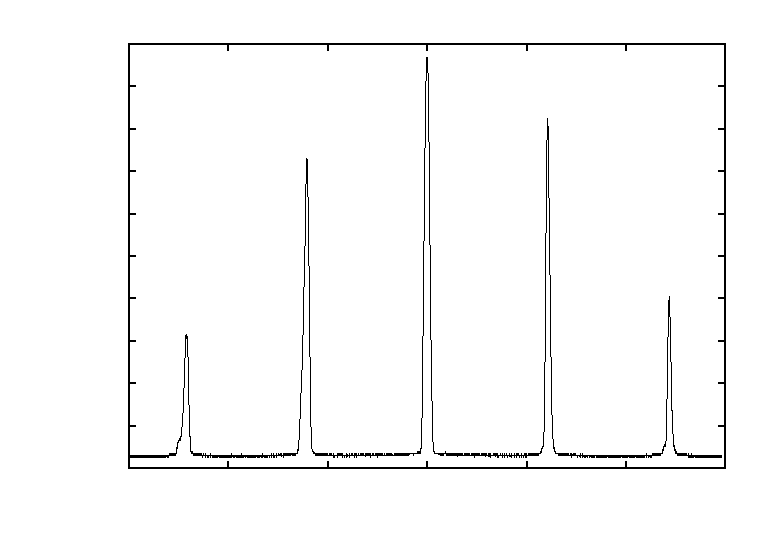
\includegraphics{g1}}%
    \gplfronttext
  \end{picture}%
\endgroup

\end{center}
\caption{Ohybový obrzec mřížky}
\label{g1}
\end{figure}

\begin{figure}
\begin{center}
% GNUPLOT: LaTeX picture with Postscript
\begingroup
  \makeatletter
  \providecommand\color[2][]{%
    \GenericError{(gnuplot) \space\space\space\@spaces}{%
      Package color not loaded in conjunction with
      terminal option `colourtext'%
    }{See the gnuplot documentation for explanation.%
    }{Either use 'blacktext' in gnuplot or load the package
      color.sty in LaTeX.}%
    \renewcommand\color[2][]{}%
  }%
  \providecommand\includegraphics[2][]{%
    \GenericError{(gnuplot) \space\space\space\@spaces}{%
      Package graphicx or graphics not loaded%
    }{See the gnuplot documentation for explanation.%
    }{The gnuplot epslatex terminal needs graphicx.sty or graphics.sty.}%
    \renewcommand\includegraphics[2][]{}%
  }%
  \providecommand\rotatebox[2]{#2}%
  \@ifundefined{ifGPcolor}{%
    \newif\ifGPcolor
    \GPcolorfalse
  }{}%
  \@ifundefined{ifGPblacktext}{%
    \newif\ifGPblacktext
    \GPblacktexttrue
  }{}%
  % define a \g@addto@macro without @ in the name:
  \let\gplgaddtomacro\g@addto@macro
  % define empty templates for all commands taking text:
  \gdef\gplbacktext{}%
  \gdef\gplfronttext{}%
  \makeatother
  \ifGPblacktext
    % no textcolor at all
    \def\colorrgb#1{}%
    \def\colorgray#1{}%
  \else
    % gray or color?
    \ifGPcolor
      \def\colorrgb#1{\color[rgb]{#1}}%
      \def\colorgray#1{\color[gray]{#1}}%
      \expandafter\def\csname LTw\endcsname{\color{white}}%
      \expandafter\def\csname LTb\endcsname{\color{black}}%
      \expandafter\def\csname LTa\endcsname{\color{black}}%
      \expandafter\def\csname LT0\endcsname{\color[rgb]{1,0,0}}%
      \expandafter\def\csname LT1\endcsname{\color[rgb]{0,1,0}}%
      \expandafter\def\csname LT2\endcsname{\color[rgb]{0,0,1}}%
      \expandafter\def\csname LT3\endcsname{\color[rgb]{1,0,1}}%
      \expandafter\def\csname LT4\endcsname{\color[rgb]{0,1,1}}%
      \expandafter\def\csname LT5\endcsname{\color[rgb]{1,1,0}}%
      \expandafter\def\csname LT6\endcsname{\color[rgb]{0,0,0}}%
      \expandafter\def\csname LT7\endcsname{\color[rgb]{1,0.3,0}}%
      \expandafter\def\csname LT8\endcsname{\color[rgb]{0.5,0.5,0.5}}%
    \else
      % gray
      \def\colorrgb#1{\color{black}}%
      \def\colorgray#1{\color[gray]{#1}}%
      \expandafter\def\csname LTw\endcsname{\color{white}}%
      \expandafter\def\csname LTb\endcsname{\color{black}}%
      \expandafter\def\csname LTa\endcsname{\color{black}}%
      \expandafter\def\csname LT0\endcsname{\color{black}}%
      \expandafter\def\csname LT1\endcsname{\color{black}}%
      \expandafter\def\csname LT2\endcsname{\color{black}}%
      \expandafter\def\csname LT3\endcsname{\color{black}}%
      \expandafter\def\csname LT4\endcsname{\color{black}}%
      \expandafter\def\csname LT5\endcsname{\color{black}}%
      \expandafter\def\csname LT6\endcsname{\color{black}}%
      \expandafter\def\csname LT7\endcsname{\color{black}}%
      \expandafter\def\csname LT8\endcsname{\color{black}}%
    \fi
  \fi
  \setlength{\unitlength}{0.0500bp}%
  \begin{picture}(7200.00,5040.00)%
    \gplgaddtomacro\gplbacktext{%
      \csname LTb\endcsname%
      \put(1078,704){\makebox(0,0)[r]{\strut{} 0}}%
      \put(1078,1286){\makebox(0,0)[r]{\strut{} 100}}%
      \put(1078,1867){\makebox(0,0)[r]{\strut{} 200}}%
      \put(1078,2449){\makebox(0,0)[r]{\strut{} 300}}%
      \put(1078,3030){\makebox(0,0)[r]{\strut{} 400}}%
      \put(1078,3612){\makebox(0,0)[r]{\strut{} 500}}%
      \put(1078,4193){\makebox(0,0)[r]{\strut{} 600}}%
      \put(1078,4775){\makebox(0,0)[r]{\strut{} 700}}%
      \put(1210,484){\makebox(0,0){\strut{}-8}}%
      \put(1917,484){\makebox(0,0){\strut{}-6}}%
      \put(2625,484){\makebox(0,0){\strut{}-4}}%
      \put(3332,484){\makebox(0,0){\strut{}-2}}%
      \put(4040,484){\makebox(0,0){\strut{} 0}}%
      \put(4747,484){\makebox(0,0){\strut{} 2}}%
      \put(5454,484){\makebox(0,0){\strut{} 4}}%
      \put(6162,484){\makebox(0,0){\strut{} 6}}%
      \put(6869,484){\makebox(0,0){\strut{} 8}}%
      \put(308,2739){\rotatebox{-270}{\makebox(0,0){\strut{}$H$/Am$^{-1}$}}}%
      \put(4039,154){\makebox(0,0){\strut{}$x$/cm}}%
    }%
    \gplgaddtomacro\gplfronttext{%
      \csname LTb\endcsname%
      \put(5882,4602){\makebox(0,0)[r]{\strut{}12 cm}}%
      \csname LTb\endcsname%
      \put(5882,4382){\makebox(0,0)[r]{\strut{}16 cm}}%
      \csname LTb\endcsname%
      \put(5882,4162){\makebox(0,0)[r]{\strut{}20 cm}}%
    }%
    \gplbacktext
    \put(0,0){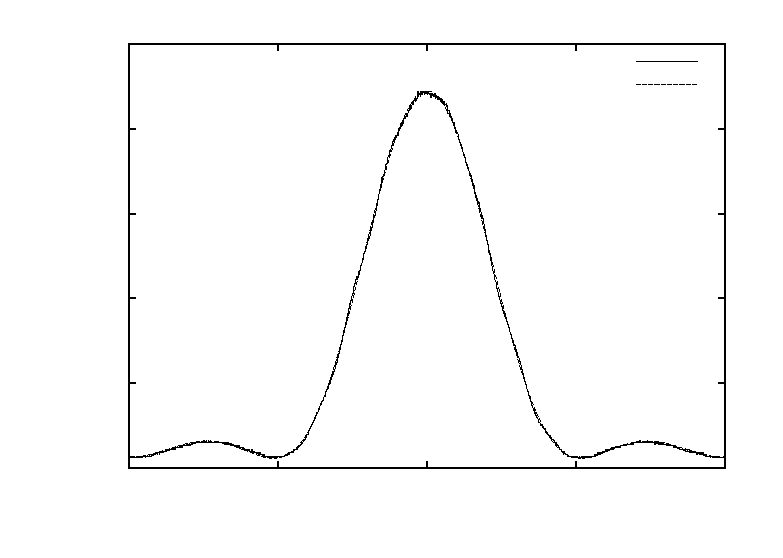
\includegraphics{g2}}%
    \gplfronttext
  \end{picture}%
\endgroup

\end{center}
\caption{Graf relativní intenzity na stínítku v závislosti na poloze pro štěrbinu A.}
\label{g2}
\end{figure}

\begin{figure}
\begin{center}
% GNUPLOT: LaTeX picture with Postscript
\begingroup
  \makeatletter
  \providecommand\color[2][]{%
    \GenericError{(gnuplot) \space\space\space\@spaces}{%
      Package color not loaded in conjunction with
      terminal option `colourtext'%
    }{See the gnuplot documentation for explanation.%
    }{Either use 'blacktext' in gnuplot or load the package
      color.sty in LaTeX.}%
    \renewcommand\color[2][]{}%
  }%
  \providecommand\includegraphics[2][]{%
    \GenericError{(gnuplot) \space\space\space\@spaces}{%
      Package graphicx or graphics not loaded%
    }{See the gnuplot documentation for explanation.%
    }{The gnuplot epslatex terminal needs graphicx.sty or graphics.sty.}%
    \renewcommand\includegraphics[2][]{}%
  }%
  \providecommand\rotatebox[2]{#2}%
  \@ifundefined{ifGPcolor}{%
    \newif\ifGPcolor
    \GPcolorfalse
  }{}%
  \@ifundefined{ifGPblacktext}{%
    \newif\ifGPblacktext
    \GPblacktexttrue
  }{}%
  % define a \g@addto@macro without @ in the name:
  \let\gplgaddtomacro\g@addto@macro
  % define empty templates for all commands taking text:
  \gdef\gplbacktext{}%
  \gdef\gplfronttext{}%
  \makeatother
  \ifGPblacktext
    % no textcolor at all
    \def\colorrgb#1{}%
    \def\colorgray#1{}%
  \else
    % gray or color?
    \ifGPcolor
      \def\colorrgb#1{\color[rgb]{#1}}%
      \def\colorgray#1{\color[gray]{#1}}%
      \expandafter\def\csname LTw\endcsname{\color{white}}%
      \expandafter\def\csname LTb\endcsname{\color{black}}%
      \expandafter\def\csname LTa\endcsname{\color{black}}%
      \expandafter\def\csname LT0\endcsname{\color[rgb]{1,0,0}}%
      \expandafter\def\csname LT1\endcsname{\color[rgb]{0,1,0}}%
      \expandafter\def\csname LT2\endcsname{\color[rgb]{0,0,1}}%
      \expandafter\def\csname LT3\endcsname{\color[rgb]{1,0,1}}%
      \expandafter\def\csname LT4\endcsname{\color[rgb]{0,1,1}}%
      \expandafter\def\csname LT5\endcsname{\color[rgb]{1,1,0}}%
      \expandafter\def\csname LT6\endcsname{\color[rgb]{0,0,0}}%
      \expandafter\def\csname LT7\endcsname{\color[rgb]{1,0.3,0}}%
      \expandafter\def\csname LT8\endcsname{\color[rgb]{0.5,0.5,0.5}}%
    \else
      % gray
      \def\colorrgb#1{\color{black}}%
      \def\colorgray#1{\color[gray]{#1}}%
      \expandafter\def\csname LTw\endcsname{\color{white}}%
      \expandafter\def\csname LTb\endcsname{\color{black}}%
      \expandafter\def\csname LTa\endcsname{\color{black}}%
      \expandafter\def\csname LT0\endcsname{\color{black}}%
      \expandafter\def\csname LT1\endcsname{\color{black}}%
      \expandafter\def\csname LT2\endcsname{\color{black}}%
      \expandafter\def\csname LT3\endcsname{\color{black}}%
      \expandafter\def\csname LT4\endcsname{\color{black}}%
      \expandafter\def\csname LT5\endcsname{\color{black}}%
      \expandafter\def\csname LT6\endcsname{\color{black}}%
      \expandafter\def\csname LT7\endcsname{\color{black}}%
      \expandafter\def\csname LT8\endcsname{\color{black}}%
    \fi
  \fi
  \setlength{\unitlength}{0.0500bp}%
  \begin{picture}(7200.00,5040.00)%
    \gplgaddtomacro\gplbacktext{%
      \csname LTb\endcsname%
      \put(1078,704){\makebox(0,0)[r]{\strut{} 100}}%
      \put(1078,1213){\makebox(0,0)[r]{\strut{} 200}}%
      \put(1078,1722){\makebox(0,0)[r]{\strut{} 300}}%
      \put(1078,2231){\makebox(0,0)[r]{\strut{} 400}}%
      \put(1078,2740){\makebox(0,0)[r]{\strut{} 500}}%
      \put(1078,3248){\makebox(0,0)[r]{\strut{} 600}}%
      \put(1078,3757){\makebox(0,0)[r]{\strut{} 700}}%
      \put(1078,4266){\makebox(0,0)[r]{\strut{} 800}}%
      \put(1078,4775){\makebox(0,0)[r]{\strut{} 900}}%
      \put(1210,484){\makebox(0,0){\strut{} 0}}%
      \put(2153,484){\makebox(0,0){\strut{} 5}}%
      \put(3096,484){\makebox(0,0){\strut{} 10}}%
      \put(4039,484){\makebox(0,0){\strut{} 15}}%
      \put(4983,484){\makebox(0,0){\strut{} 20}}%
      \put(5926,484){\makebox(0,0){\strut{} 25}}%
      \put(6869,484){\makebox(0,0){\strut{} 30}}%
      \put(308,2739){\rotatebox{-270}{\makebox(0,0){\strut{}$R/\Omega$}}}%
      \put(4039,154){\makebox(0,0){\strut{}$I/$mA}}%
    }%
    \gplgaddtomacro\gplfronttext{%
      \csname LTb\endcsname%
      \put(4774,4602){\makebox(0,0)[r]{\strut{}substituční metoda}}%
      \csname LTb\endcsname%
      \put(4774,4382){\makebox(0,0)[r]{\strut{}přímá metoda s korekcí}}%
    }%
    \gplbacktext
    \put(0,0){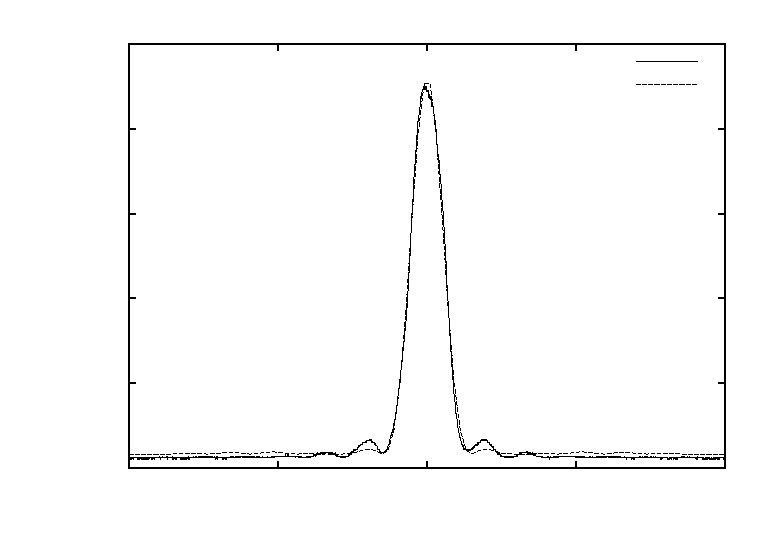
\includegraphics{g3}}%
    \gplfronttext
  \end{picture}%
\endgroup

\end{center}
\caption{Graf relativní intenzity na stínítku v závislosti na poloze pro štěrbinu C.}
\label{g3}
\end{figure}

\begin{figure}
\begin{center}
% GNUPLOT: LaTeX picture with Postscript
\begingroup
  \makeatletter
  \providecommand\color[2][]{%
    \GenericError{(gnuplot) \space\space\space\@spaces}{%
      Package color not loaded in conjunction with
      terminal option `colourtext'%
    }{See the gnuplot documentation for explanation.%
    }{Either use 'blacktext' in gnuplot or load the package
      color.sty in LaTeX.}%
    \renewcommand\color[2][]{}%
  }%
  \providecommand\includegraphics[2][]{%
    \GenericError{(gnuplot) \space\space\space\@spaces}{%
      Package graphicx or graphics not loaded%
    }{See the gnuplot documentation for explanation.%
    }{The gnuplot epslatex terminal needs graphicx.sty or graphics.sty.}%
    \renewcommand\includegraphics[2][]{}%
  }%
  \providecommand\rotatebox[2]{#2}%
  \@ifundefined{ifGPcolor}{%
    \newif\ifGPcolor
    \GPcolorfalse
  }{}%
  \@ifundefined{ifGPblacktext}{%
    \newif\ifGPblacktext
    \GPblacktexttrue
  }{}%
  % define a \g@addto@macro without @ in the name:
  \let\gplgaddtomacro\g@addto@macro
  % define empty templates for all commands taking text:
  \gdef\gplbacktext{}%
  \gdef\gplfronttext{}%
  \makeatother
  \ifGPblacktext
    % no textcolor at all
    \def\colorrgb#1{}%
    \def\colorgray#1{}%
  \else
    % gray or color?
    \ifGPcolor
      \def\colorrgb#1{\color[rgb]{#1}}%
      \def\colorgray#1{\color[gray]{#1}}%
      \expandafter\def\csname LTw\endcsname{\color{white}}%
      \expandafter\def\csname LTb\endcsname{\color{black}}%
      \expandafter\def\csname LTa\endcsname{\color{black}}%
      \expandafter\def\csname LT0\endcsname{\color[rgb]{1,0,0}}%
      \expandafter\def\csname LT1\endcsname{\color[rgb]{0,1,0}}%
      \expandafter\def\csname LT2\endcsname{\color[rgb]{0,0,1}}%
      \expandafter\def\csname LT3\endcsname{\color[rgb]{1,0,1}}%
      \expandafter\def\csname LT4\endcsname{\color[rgb]{0,1,1}}%
      \expandafter\def\csname LT5\endcsname{\color[rgb]{1,1,0}}%
      \expandafter\def\csname LT6\endcsname{\color[rgb]{0,0,0}}%
      \expandafter\def\csname LT7\endcsname{\color[rgb]{1,0.3,0}}%
      \expandafter\def\csname LT8\endcsname{\color[rgb]{0.5,0.5,0.5}}%
    \else
      % gray
      \def\colorrgb#1{\color{black}}%
      \def\colorgray#1{\color[gray]{#1}}%
      \expandafter\def\csname LTw\endcsname{\color{white}}%
      \expandafter\def\csname LTb\endcsname{\color{black}}%
      \expandafter\def\csname LTa\endcsname{\color{black}}%
      \expandafter\def\csname LT0\endcsname{\color{black}}%
      \expandafter\def\csname LT1\endcsname{\color{black}}%
      \expandafter\def\csname LT2\endcsname{\color{black}}%
      \expandafter\def\csname LT3\endcsname{\color{black}}%
      \expandafter\def\csname LT4\endcsname{\color{black}}%
      \expandafter\def\csname LT5\endcsname{\color{black}}%
      \expandafter\def\csname LT6\endcsname{\color{black}}%
      \expandafter\def\csname LT7\endcsname{\color{black}}%
      \expandafter\def\csname LT8\endcsname{\color{black}}%
    \fi
  \fi
  \setlength{\unitlength}{0.0500bp}%
  \begin{picture}(7200.00,5040.00)%
    \gplgaddtomacro\gplbacktext{%
      \csname LTb\endcsname%
      \put(946,1010){\makebox(0,0)[r]{\strut{} 20}}%
      \put(946,1481){\makebox(0,0)[r]{\strut{} 40}}%
      \put(946,1951){\makebox(0,0)[r]{\strut{} 60}}%
      \put(946,2422){\makebox(0,0)[r]{\strut{} 80}}%
      \put(946,2892){\makebox(0,0)[r]{\strut{} 100}}%
      \put(946,3363){\makebox(0,0)[r]{\strut{} 120}}%
      \put(946,3834){\makebox(0,0)[r]{\strut{} 140}}%
      \put(946,4304){\makebox(0,0)[r]{\strut{} 160}}%
      \put(946,4775){\makebox(0,0)[r]{\strut{} 180}}%
      \put(1078,484){\makebox(0,0){\strut{} 790}}%
      \put(2032,484){\makebox(0,0){\strut{} 800}}%
      \put(2986,484){\makebox(0,0){\strut{} 810}}%
      \put(3941,484){\makebox(0,0){\strut{} 820}}%
      \put(4895,484){\makebox(0,0){\strut{} 830}}%
      \put(5849,484){\makebox(0,0){\strut{} 840}}%
      \put(6803,484){\makebox(0,0){\strut{} 850}}%
      \put(176,2739){\rotatebox{-270}{\makebox(0,0){\strut{}rel. intenzita}}}%
      \put(3940,154){\makebox(0,0){\strut{}$\lambda$/nm}}%
    }%
    \gplgaddtomacro\gplfronttext{%
      \csname LTb\endcsname%
      \put(5816,4602){\makebox(0,0)[r]{\strut{}80.0 mA}}%
      \csname LTb\endcsname%
      \put(5816,4382){\makebox(0,0)[r]{\strut{}90.1 mA}}%
      \csname LTb\endcsname%
      \put(5816,4162){\makebox(0,0)[r]{\strut{}100.2 mA}}%
      \csname LTb\endcsname%
      \put(5816,3942){\makebox(0,0)[r]{\strut{}110.1 mA}}%
      \csname LTb\endcsname%
      \put(5816,3722){\makebox(0,0)[r]{\strut{}114.3 mA}}%
    }%
    \gplbacktext
    \put(0,0){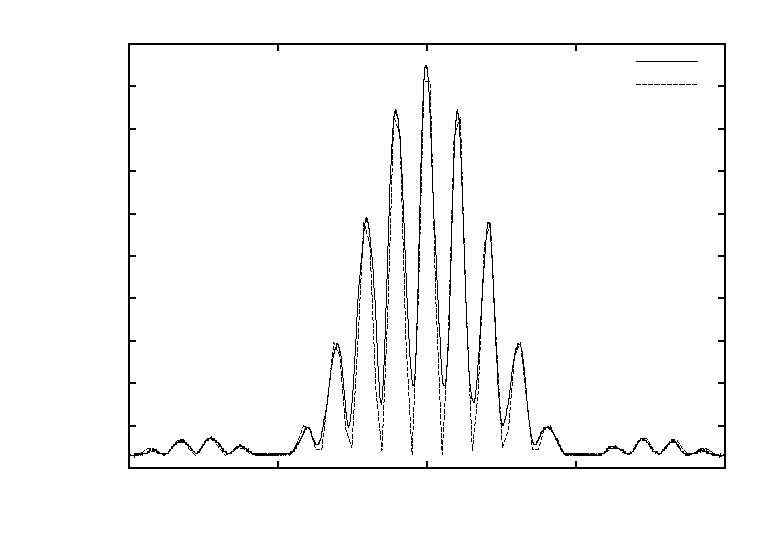
\includegraphics{g4}}%
    \gplfronttext
  \end{picture}%
\endgroup

\end{center}
\caption{Graf relativní intenzity na stínítku v závislosti na poloze pro dvojštěrbinu A.}
\label{g4}
\end{figure}

\begin{figure}
\begin{center}
% GNUPLOT: LaTeX picture with Postscript
\begingroup
  \makeatletter
  \providecommand\color[2][]{%
    \GenericError{(gnuplot) \space\space\space\@spaces}{%
      Package color not loaded in conjunction with
      terminal option `colourtext'%
    }{See the gnuplot documentation for explanation.%
    }{Either use 'blacktext' in gnuplot or load the package
      color.sty in LaTeX.}%
    \renewcommand\color[2][]{}%
  }%
  \providecommand\includegraphics[2][]{%
    \GenericError{(gnuplot) \space\space\space\@spaces}{%
      Package graphicx or graphics not loaded%
    }{See the gnuplot documentation for explanation.%
    }{The gnuplot epslatex terminal needs graphicx.sty or graphics.sty.}%
    \renewcommand\includegraphics[2][]{}%
  }%
  \providecommand\rotatebox[2]{#2}%
  \@ifundefined{ifGPcolor}{%
    \newif\ifGPcolor
    \GPcolorfalse
  }{}%
  \@ifundefined{ifGPblacktext}{%
    \newif\ifGPblacktext
    \GPblacktexttrue
  }{}%
  % define a \g@addto@macro without @ in the name:
  \let\gplgaddtomacro\g@addto@macro
  % define empty templates for all commands taking text:
  \gdef\gplbacktext{}%
  \gdef\gplfronttext{}%
  \makeatother
  \ifGPblacktext
    % no textcolor at all
    \def\colorrgb#1{}%
    \def\colorgray#1{}%
  \else
    % gray or color?
    \ifGPcolor
      \def\colorrgb#1{\color[rgb]{#1}}%
      \def\colorgray#1{\color[gray]{#1}}%
      \expandafter\def\csname LTw\endcsname{\color{white}}%
      \expandafter\def\csname LTb\endcsname{\color{black}}%
      \expandafter\def\csname LTa\endcsname{\color{black}}%
      \expandafter\def\csname LT0\endcsname{\color[rgb]{1,0,0}}%
      \expandafter\def\csname LT1\endcsname{\color[rgb]{0,1,0}}%
      \expandafter\def\csname LT2\endcsname{\color[rgb]{0,0,1}}%
      \expandafter\def\csname LT3\endcsname{\color[rgb]{1,0,1}}%
      \expandafter\def\csname LT4\endcsname{\color[rgb]{0,1,1}}%
      \expandafter\def\csname LT5\endcsname{\color[rgb]{1,1,0}}%
      \expandafter\def\csname LT6\endcsname{\color[rgb]{0,0,0}}%
      \expandafter\def\csname LT7\endcsname{\color[rgb]{1,0.3,0}}%
      \expandafter\def\csname LT8\endcsname{\color[rgb]{0.5,0.5,0.5}}%
    \else
      % gray
      \def\colorrgb#1{\color{black}}%
      \def\colorgray#1{\color[gray]{#1}}%
      \expandafter\def\csname LTw\endcsname{\color{white}}%
      \expandafter\def\csname LTb\endcsname{\color{black}}%
      \expandafter\def\csname LTa\endcsname{\color{black}}%
      \expandafter\def\csname LT0\endcsname{\color{black}}%
      \expandafter\def\csname LT1\endcsname{\color{black}}%
      \expandafter\def\csname LT2\endcsname{\color{black}}%
      \expandafter\def\csname LT3\endcsname{\color{black}}%
      \expandafter\def\csname LT4\endcsname{\color{black}}%
      \expandafter\def\csname LT5\endcsname{\color{black}}%
      \expandafter\def\csname LT6\endcsname{\color{black}}%
      \expandafter\def\csname LT7\endcsname{\color{black}}%
      \expandafter\def\csname LT8\endcsname{\color{black}}%
    \fi
  \fi
  \setlength{\unitlength}{0.0500bp}%
  \begin{picture}(7200.00,5040.00)%
    \gplgaddtomacro\gplbacktext{%
      \csname LTb\endcsname%
      \put(946,704){\makebox(0,0)[r]{\strut{} 40}}%
      \put(946,1213){\makebox(0,0)[r]{\strut{} 60}}%
      \put(946,1722){\makebox(0,0)[r]{\strut{} 80}}%
      \put(946,2231){\makebox(0,0)[r]{\strut{} 100}}%
      \put(946,2740){\makebox(0,0)[r]{\strut{} 120}}%
      \put(946,3248){\makebox(0,0)[r]{\strut{} 140}}%
      \put(946,3757){\makebox(0,0)[r]{\strut{} 160}}%
      \put(946,4266){\makebox(0,0)[r]{\strut{} 180}}%
      \put(946,4775){\makebox(0,0)[r]{\strut{} 200}}%
      \put(1078,484){\makebox(0,0){\strut{} 795}}%
      \put(1714,484){\makebox(0,0){\strut{} 800}}%
      \put(2350,484){\makebox(0,0){\strut{} 805}}%
      \put(2986,484){\makebox(0,0){\strut{} 810}}%
      \put(3622,484){\makebox(0,0){\strut{} 815}}%
      \put(4259,484){\makebox(0,0){\strut{} 820}}%
      \put(4895,484){\makebox(0,0){\strut{} 825}}%
      \put(5531,484){\makebox(0,0){\strut{} 830}}%
      \put(6167,484){\makebox(0,0){\strut{} 835}}%
      \put(6803,484){\makebox(0,0){\strut{} 840}}%
      \put(176,2739){\rotatebox{-270}{\makebox(0,0){\strut{}relativní intenzita}}}%
      \put(3940,154){\makebox(0,0){\strut{}$\lambda$/nm}}%
    }%
    \gplgaddtomacro\gplfronttext{%
      \csname LTb\endcsname%
      \put(5816,4602){\makebox(0,0)[r]{\strut{}první měřnení}}%
      \csname LTb\endcsname%
      \put(5816,4382){\makebox(0,0)[r]{\strut{}druhé měření}}%
    }%
    \gplbacktext
    \put(0,0){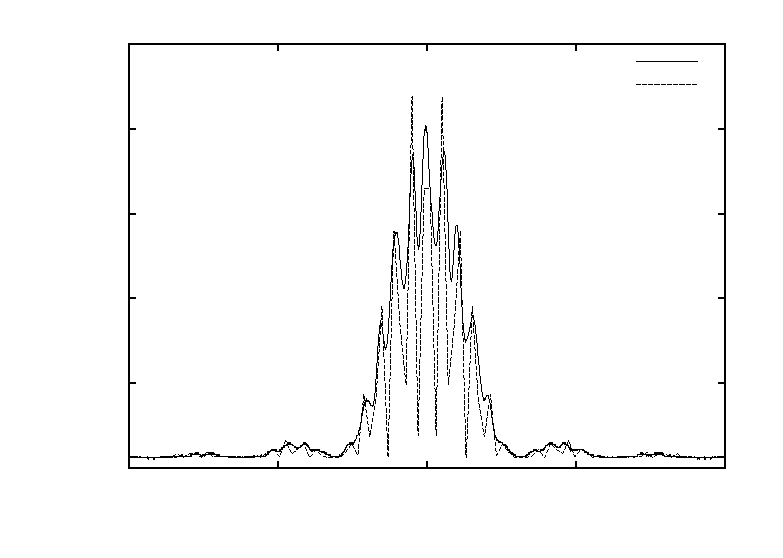
\includegraphics{g5}}%
    \gplfronttext
  \end{picture}%
\endgroup

\end{center}
\caption{Graf relativní intenzity na stínítku v závislosti na poloze pro dvojštěrbinu C.}
\label{g5}
\end{figure}

\begin{figure}
\begin{center}
% GNUPLOT: LaTeX picture with Postscript
\begingroup
  \makeatletter
  \providecommand\color[2][]{%
    \GenericError{(gnuplot) \space\space\space\@spaces}{%
      Package color not loaded in conjunction with
      terminal option `colourtext'%
    }{See the gnuplot documentation for explanation.%
    }{Either use 'blacktext' in gnuplot or load the package
      color.sty in LaTeX.}%
    \renewcommand\color[2][]{}%
  }%
  \providecommand\includegraphics[2][]{%
    \GenericError{(gnuplot) \space\space\space\@spaces}{%
      Package graphicx or graphics not loaded%
    }{See the gnuplot documentation for explanation.%
    }{The gnuplot epslatex terminal needs graphicx.sty or graphics.sty.}%
    \renewcommand\includegraphics[2][]{}%
  }%
  \providecommand\rotatebox[2]{#2}%
  \@ifundefined{ifGPcolor}{%
    \newif\ifGPcolor
    \GPcolorfalse
  }{}%
  \@ifundefined{ifGPblacktext}{%
    \newif\ifGPblacktext
    \GPblacktexttrue
  }{}%
  % define a \g@addto@macro without @ in the name:
  \let\gplgaddtomacro\g@addto@macro
  % define empty templates for all commands taking text:
  \gdef\gplbacktext{}%
  \gdef\gplfronttext{}%
  \makeatother
  \ifGPblacktext
    % no textcolor at all
    \def\colorrgb#1{}%
    \def\colorgray#1{}%
  \else
    % gray or color?
    \ifGPcolor
      \def\colorrgb#1{\color[rgb]{#1}}%
      \def\colorgray#1{\color[gray]{#1}}%
      \expandafter\def\csname LTw\endcsname{\color{white}}%
      \expandafter\def\csname LTb\endcsname{\color{black}}%
      \expandafter\def\csname LTa\endcsname{\color{black}}%
      \expandafter\def\csname LT0\endcsname{\color[rgb]{1,0,0}}%
      \expandafter\def\csname LT1\endcsname{\color[rgb]{0,1,0}}%
      \expandafter\def\csname LT2\endcsname{\color[rgb]{0,0,1}}%
      \expandafter\def\csname LT3\endcsname{\color[rgb]{1,0,1}}%
      \expandafter\def\csname LT4\endcsname{\color[rgb]{0,1,1}}%
      \expandafter\def\csname LT5\endcsname{\color[rgb]{1,1,0}}%
      \expandafter\def\csname LT6\endcsname{\color[rgb]{0,0,0}}%
      \expandafter\def\csname LT7\endcsname{\color[rgb]{1,0.3,0}}%
      \expandafter\def\csname LT8\endcsname{\color[rgb]{0.5,0.5,0.5}}%
    \else
      % gray
      \def\colorrgb#1{\color{black}}%
      \def\colorgray#1{\color[gray]{#1}}%
      \expandafter\def\csname LTw\endcsname{\color{white}}%
      \expandafter\def\csname LTb\endcsname{\color{black}}%
      \expandafter\def\csname LTa\endcsname{\color{black}}%
      \expandafter\def\csname LT0\endcsname{\color{black}}%
      \expandafter\def\csname LT1\endcsname{\color{black}}%
      \expandafter\def\csname LT2\endcsname{\color{black}}%
      \expandafter\def\csname LT3\endcsname{\color{black}}%
      \expandafter\def\csname LT4\endcsname{\color{black}}%
      \expandafter\def\csname LT5\endcsname{\color{black}}%
      \expandafter\def\csname LT6\endcsname{\color{black}}%
      \expandafter\def\csname LT7\endcsname{\color{black}}%
      \expandafter\def\csname LT8\endcsname{\color{black}}%
    \fi
  \fi
  \setlength{\unitlength}{0.0500bp}%
  \begin{picture}(7200.00,5040.00)%
    \gplgaddtomacro\gplbacktext{%
      \csname LTb\endcsname%
      \put(594,440){\makebox(0,0)[r]{\strut{} 0}}%
      \put(594,874){\makebox(0,0)[r]{\strut{} 1}}%
      \put(594,1307){\makebox(0,0)[r]{\strut{} 2}}%
      \put(594,1741){\makebox(0,0)[r]{\strut{} 3}}%
      \put(594,2174){\makebox(0,0)[r]{\strut{} 4}}%
      \put(594,2608){\makebox(0,0)[r]{\strut{} 5}}%
      \put(594,3041){\makebox(0,0)[r]{\strut{} 6}}%
      \put(594,3475){\makebox(0,0)[r]{\strut{} 7}}%
      \put(594,3908){\makebox(0,0)[r]{\strut{} 8}}%
      \put(594,4342){\makebox(0,0)[r]{\strut{} 9}}%
      \put(594,4775){\makebox(0,0)[r]{\strut{} 10}}%
      \put(726,220){\makebox(0,0){\strut{} 0}}%
      \put(1486,220){\makebox(0,0){\strut{} 0.2}}%
      \put(2245,220){\makebox(0,0){\strut{} 0.4}}%
      \put(3005,220){\makebox(0,0){\strut{} 0.6}}%
      \put(3765,220){\makebox(0,0){\strut{} 0.8}}%
      \put(4524,220){\makebox(0,0){\strut{} 1}}%
      \put(5284,220){\makebox(0,0){\strut{} 1.2}}%
      \put(6043,220){\makebox(0,0){\strut{} 1.4}}%
      \put(6803,220){\makebox(0,0){\strut{} 1.6}}%
    }%
    \gplgaddtomacro\gplfronttext{%
      \csname LTb\endcsname%
      \put(5816,613){\makebox(0,0)[r]{\strut{}kalibrační křivka}}%
    }%
    \gplbacktext
    \put(0,0){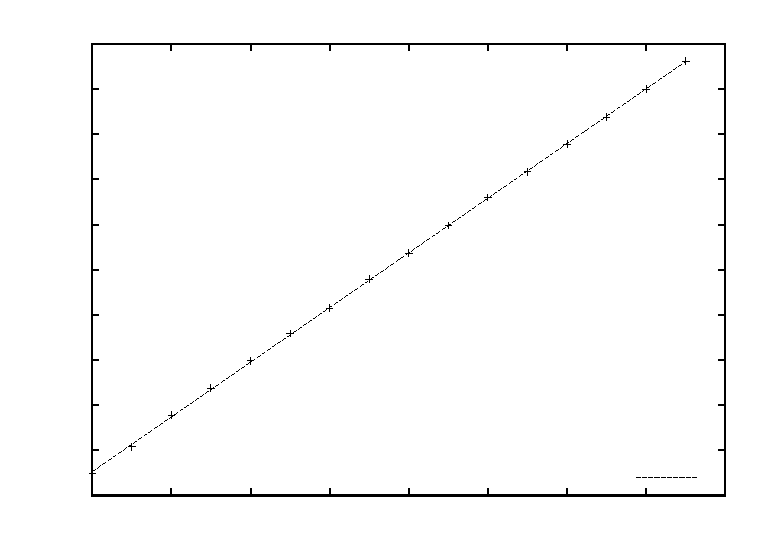
\includegraphics{kal}}%
    \gplfronttext
  \end{picture}%
\endgroup

\end{center}
\caption{Kalibrační křivka mikroskopu.}
\label{kal}
\end{figure}


\eject
\begin{thebibliography}{5}
	\bibitem{text} \textbf{Studijní text na praktikum III} \\http://physics.mff.cuni.cz/vyuka/zfp/txt\_306.htm (8. 3. 2012)
    \bibitem{chyba} \emph{J. Englich}: \textbf{Zpracování výsldků fyzikálních měření} \\ LS 1999/2000
    \bibitem{maly} \emph{prof. RNDr. Petr Malý , DrSc.}: \textbf{Optika}\\Univerzita Karlova v Praze, Nakladatelství Karolinum 2008, první vydání
\end{thebibliography}



\end{document}
